% Komentārs: oriģināla metodika, mērījumu/aprēķinu precizitātes novērtējums

\section{Tipi} \label{section:tipi}

% Rindkopa par to, kādi materiāli un ka ir mono un polikristāli un monokristāli labāki un kāpēc.

Botāniskā dārza saules paneļu sistēmu raksturo divi saules paneļu tipi -- JA un LG. Šajā nodaļā saules paneļu tipi tiek salīdzināti savā starpā, gan apskatīti kontekstā ar maksimālo teorētisko efektivitāti.

Ideāli efektīva saules šūna uzņem un iesloga visu krītošo gaismu un 
konvertē to elektriskajos nesējos, kas tiek efektīvi savākti, reālās saules šūnas ir nepilnīgas vienā vai abos no šiem aspektiem. Fundamentālās saules šūnu efektivitātes robeža pēc Šokleja-Ķoizera (\textit{Shockley-Queisser}, S-Q) detalizētā balansa modeļa ir 33.7\%, balstoties uz modeli monokristālisks Si ir sasniedzis $>75\%$ no S-Q robežas, bet polikristālisks Si $50$ līdz $75\%$ no S-Q robežas~\cite{polman2016}.

Monokristāla Si šūnu efektivitātes rekords ir 25.6\%, tās ir sasniegušas gandrīz pilnīgu gaismas slazdošanu un nesēju savākšanu, un lielākoties tās ierobežo nesēja rekombinācijas zudumi. Polikristālisko Si šūnu efektivitātes rekords ir 21.3\%.
% moduļa eff 18.5\%
Polikristālisks Si pusvadītāja plāksnes tiek izgrieztas no stieņa ar virzītās kristalizācijas metodi, un to izgatavošanas izmaksas ir mazākas nekā monokristāliskām plāksnēm. Taču polikristāliskam Si ir zemāka elektroniskā kvalitāte kristāla graudu robežu un iekšgraudu defektu dēļ, kā arī lielāka piemaisījumu koncentrācija, tāpēc polikristāliskai saules šūnai ir lieli sprieguma zudumi. Gaismas slazdošana šajās šūnās ir mazāk efektīva, jo ideālā piramīdas virsmas tekstūra, ko parasti izveido sārmainā kodināšana Si(100) uz (111) virsmas plaknēm, nevar realizēties polikristāliskā virsmā~\cite{polman2016}.
% alkaline-etching Si(100) to (111) surface facets cannot be realized on a multicrystalline surface
% Kontakta rekombinācija reprezentē lielāko daļu zudumu, tāpēc veiksmīgākie risinājumi minimizē saskarsmes laukumu (piem., lokalizēta heavy doping or metal seposition), implementē pasivētus kontkatus vai izmanto šo paņēmienu kombināciju.

Ražotāju referenču lapās LG tiek prognozēta labāka atdeve saulainās dienās~\cite{LGtips}, bet JA labāka atdeve vājas gaismas intensitātes apstākļos~\cite{JAtips}. Ņemot vērā nespēju šos apgalvojumu patiesumu praktiski pārbaudīt patentēto (\textit{proprietary}) modeļu dēļ, atsevišķi izvērtējot tikai \ref{section:clouds}. nod. aprakstītos mākoņainības apsvērumus, Latvijas klimatam piemērotāks būtu JA.

\begin{table}[h]
    \caption{JA un LG paneļu tipu salīdzinājums~\cite{JAtips}~\cite{LGtips}} % uzrakstīt kādu absolūto TSI izmērīja vai norādīt uz grafiku?
    \begin{center}
    \begin{tabular}{| r | c | c |}
    \hline
    Tipa abreviatūra & JA & LG \\ \hline
    Modelis &  JAP60-275/4BB & LG365Q1C-A5\\ \hline
    % materiāls & silikons &   \\ \hline
	Kristāla veids & Polikristālisks & Monokristālisks \\ \hline
	% šūnas izmērs, mm  &156x156  & \\ \hline
	Šūnu skaits  &60  &60 \\ \hline
	Virsmas laukums, $m^2$ &1.64  &1.72 \\ \hline
	STC Pmax, $W$ 	&270 &365\\ \hline
	NOCT Pmax, $W$  &196 &275\\ \hline
	Efektivitāte, \% &16 & 20\\ \hline
    \end{tabular}
    \end{center}
    \label{tab:ja_lg_tipi}
\end{table}

Paneļu maksimālā jauda ($P_{max}$) tiek testēta pie:
\begin{itemize}
\item standarta testa nosacījumiem (\textit{Standart test condition} - STC):\\
Saules izstarojums 1000 W/m$^2$; apkārtējā temperatūra 25\textdegree C.
\item nominālās šūnas darba temperatūras (\textit{Nominal operating cell temperature} - NOCT):\\
Saules izstarojums 800 W/m$^2$; apkārtējā temperatūra 20 \textdegree C; vēja ātrums 1 m/s
\end{itemize}

% ielikt bildi ar to kas saules apstarojumā pazūd no imene

\section{Elektriskā shēma}

Šajā nodaļā tiek paskaidrotas elektroniskās shēmas (skat.\ref{fig:shema}.att.) komponentes un to funkcionalitāte.

\begin{enumerate}
\item Saules baterijas (skat. ~\ref{section:mechanism}. un ~\ref{section:tipi}. nodaļas)
\item \emph{SmartSolar MPPT} --
Saules enerģijas lādētājs savāc enerģiju no saules bateriju paneļiem un noglabā to akumulatoros. Tā mērķis ir novērst bateriju izlādēšanās izraisītos bojājumus. Pirmais skaitlis modeļa nosaukumā apzīmē maksimālo PV slēguma spriegumu, otrais -- maksimālo uzlādes strāvu.
\item Līdzstrāvas drošinātāju skapis -- nepieciešamības gadījumā izolē slēgumu no barošanas avota.
\item \emph{Cyrix-Li-Charge 12/24V -120 A} --
Lādēšanas ierobežotājs atslēdzas, kad tā kontroles izvade kļūs brīvi peldoša (\textit{free floathing}), signalizējot par baterijas pārspriegumu vai paaugstinātu temperatūru. Tas pievieno akumulatora lādētāju ar 3 sekunžu aizkavi, ja VE.Bus BMS lādiņa atvienošanas (\textit{Charge Disconnect}) izvade ir augsta (\textit{high}), spriegums uz akumulatora lādētāja savienojuma spailes ir $\geq 13.7$ V vai spriegums uz akumulatora spailes ir $\geq 2$V.
\item Kūstošais drošinātais --
izkūst pārslodzes gadījumā, novēršot dārgāku instrumentu bojāšanu.
\item \emph{LiFeO4 akumulators 13.8V/90Ah - BMS}
\item Šunts -- mazas pretestības ceļš, ko pieslēdz paralēli galvenajam elektriskās ķēdes posmam, lai tajā samazinātu strāvu. PV sistēmās lietots, lai apietu nevēlamu īssavienojumu starp saules baterijas priekšējo un aizmugurējo virsmas kontaktu, ko parasti izraisa pusvadītāja plāksnes bojājumi.
\item \emph{BMV-702 Smart} --
Akumulatora monitors aprēķina akumulatora spriegumu, strāvas stiprumu, patērēto ampērstundu skaitu, uzlādes stāvokli un atlikušo sistēmas darbības laiku pie pašreizējās izlādes ātruma.
\item \emph{VE.BUS BMS} --
Bateriju vadības bloks pasargā no akumulatoru bojājumiem uzlādes nelīdzsvatorības dēļ. Baterija ar nedaudz lielāku iekšējās noplūdes strāvu
%bateriju bankā ar daudzām virknē vai paralēli savienotām baterijām
izraisīs konkrētās baterijas un paralēli savienoto bateriju nepietiekamu uzlādi un virknē savienoto bateriju pārlādi. Taču virknē savienotām baterijām nepieciešams vienāds sākotnējais uzlādes līmenis. Mazas atšķirības uzlādes līmenī tiks novērstas absorbcijas vai izlīdzināšanās ceļā, bet lielas atšķirības izraisīs bojājumus pārmērīgas pārlādes izraisītas gazifikācijas dēļ baterijām ar lielāku sākotnējo uzlādes līmeni un nepietiekamas uzlādes izraisītās sulfācijas dēļ baterijām ar mazāku sākotnējo uzlādes līmeni.

Bateriju vadības bloks pielīdzina uzlādes līmeni divām bateriju virknēm vai daudzām paralēli savienotām bateriju virknēm. Kad uzlādes spriegums bateriju sistēmai palielinās līdz sistēmā iestatītajai robežai, baterijas vadības bloks salīdzina spriegumus divās virknēs savienotajās baterijās un samazina strāvas padevi akumulatoram (vai paralēli savienotām baterijām) ar augstāko spriegumu. Rezultātā izveidotais uzlādes strāvas diferenciālis nodrošinās, ka visas baterijas konverģēs vienā uzlādes stāvoklī.
% http://www.ultraflexgroup.com/en/catalogue/batteries/09909d-1/1170/vebus-bms.html
% sulfācija - Organiskā savienojuma ūdeņraža atoma aizstāšana ar sulfāta (- OSO2OH) funkcionālo grupu vai divu molekulu ūdeņraža atomu aizstāšana, lai veidotu sulfātu (R-OSO2O-R)
\item \emph{Octo GX} -- instalācijas sakaru centrs ar tālvadības konsoli tiešraides datu uzraudzībai un iestatījumu maiņai, kurai var piekļūt caur Victorn Attālinātās Pārvaldības Portālu(\textit{Victron Remote Management Portal}, VRM) vai lokālo LAN/WiFI tīklu.
% The Octo GX is particularly suited to medium size installations which have many MPPT Solar Chargers, as it has 10 VE.Direct ports
\item \emph{MultiPlus 24/3000/70-16 230V VE.Bus}  --
Autonoms lādētājs pārņēm strāvas padevi tīkla avārijas vai ģeneratora strāva atvienošanās gadījumā $<20$ ms laikā, lai elektroniskās iekārtas turpina darboties bez traucējumiem~\cite{victron}. 
\end{enumerate}

\begin{figure}[h]
    \centering
    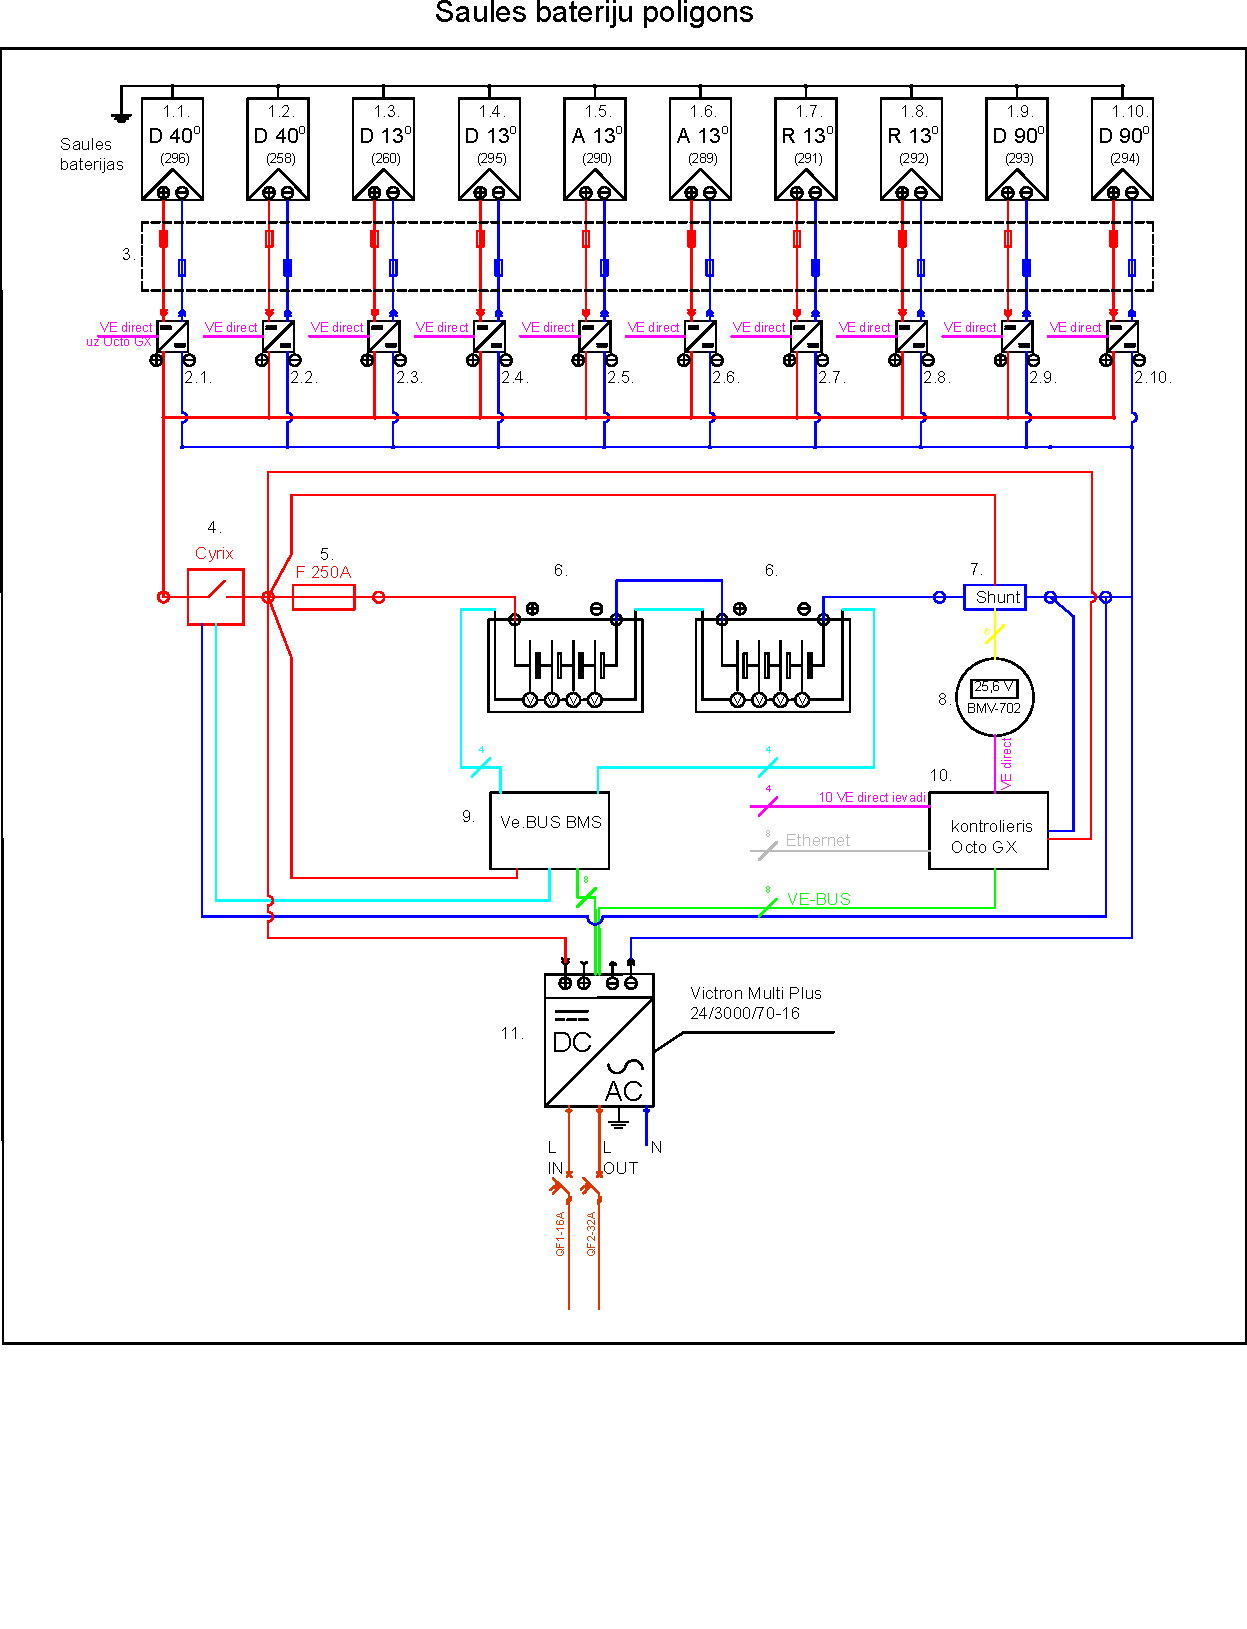
\includegraphics[width=0.7\linewidth]{figures/misc/shema.pdf}
    \caption{Saules paneļu elektriskā shēma (autors Valdis Gailītis, modifikācijas Viktorija Leimane)}
    \label{fig:shema}
\end{figure}

\section{Telpiskās orientācijas}

Pēc telpiskās orientācijas saules paneļi tiek iedalīti divās grupās:
\begin{itemize}
\item 13 grādu leņķī (R13, A13, D13)
\item D virzienā (D13, D40, D90)
\end{itemize}

LU Botāniskā dārzā uzstādīto saules paneļu telpiskās orientācijas uzskatāmi parādītas \ref{fig:paneli}. att. (shematiski) un \ref{fig:paneli2}. att. (dabā). Lai lasītājam atvieglotu rezultātu interpretāciju, šīs grupas grafikos tiek apzinātas ar krāsām: leņķu grupa tiek apzīmēta ar zaļo krāsu, D virziena grupa ar zilo, abām grupām kopīgais panelis D13 -- ar tirkīzzilu, krāsu paletes leģenda pieejama \ref{fig:paneli}. att.


\begin{figure}[h]
    \centering
    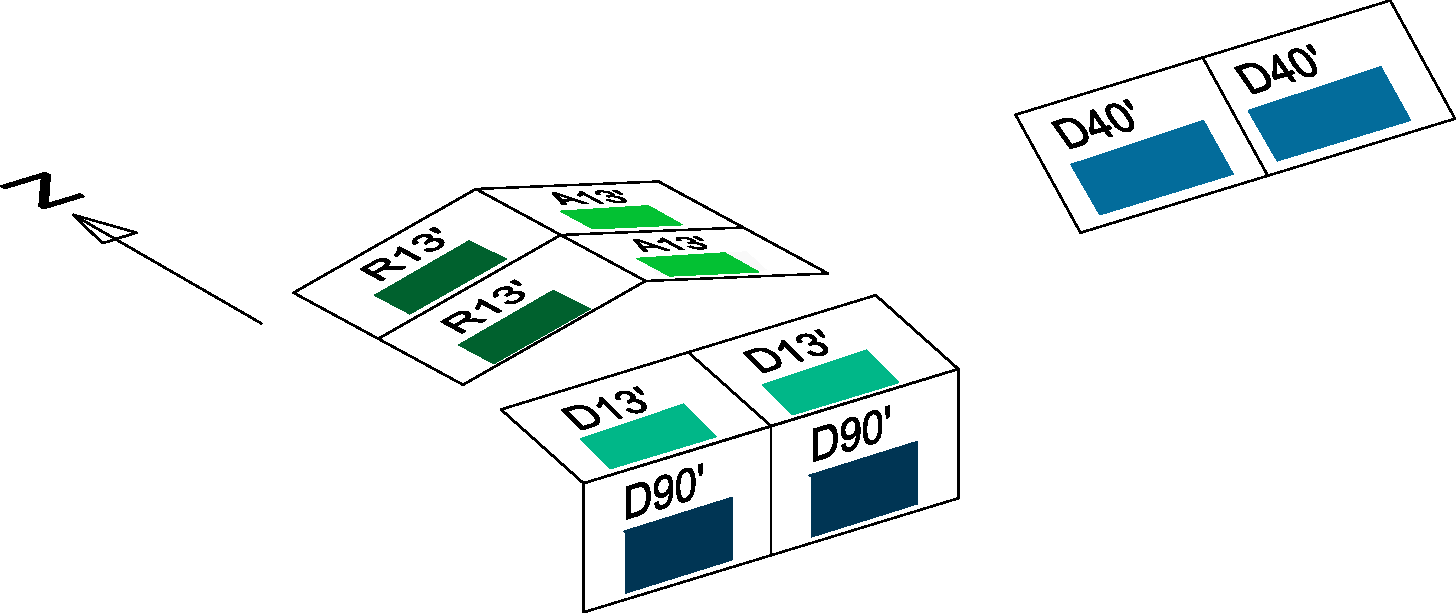
\includegraphics[width=0.7\linewidth]{figures/misc/krasas_izvietojums.pdf}
    \caption{Saules paneļu telpisko orientāciju shēma (autors Valdis Gailītis, modifikācijas Viktorija Leimane)}
    \label{fig:paneli}
\end{figure}

\begin{figure}[h]
    \centering
    \includegraphics[width=0.7\linewidth]{figures/stenduBildes/overview2.JPG}
    \caption{Saules paneļu telpiskās orientācijas dabā (fotogrāfijas autors Māris Šinka)}
    \label{fig:paneli2}
\end{figure}